\chapter{L'Energia}
\section{Lavoro}
\begin{defi}
	Il lavoro è definito come il prodotto della forza per lo spostamento del
	suo punto di applicazione. Esso è quindi uno scalare
	\begin{equation}
		L=\vec{F}*\vec{s}=Fs\cos \theta
	\end{equation}
	In cui $\theta$ è l'angolo più piccolo formato tra la forza e lo
	spostamento
	\begin{equation*}
		\begin{matrix}
			\text{Dimensioni: } & [L]=[F][L]=[MLT^{-2}][l]=[ML^2T^{-2}]\\
			\text{Unita in misura: } & Kg m^2 s^{-2} = \text{Joule simbolo (J)}
		\end{matrix}
	\end{equation*}
	$L=\vec{F}*\vec{s}=Fs\cos\theta$
	\begin{equation*}
		\begin{matrix}
			L>0 &\Rightarrow \cos \theta>0 &\Rightarrow \theta < \frac{\pi}{2}=90^o\\
			L=0 &\Rightarrow \cos \theta=0 &\Rightarrow \theta =
			\frac{\pi}{2}\\
			L<0& \Rightarrow \cos \theta <0 & \Rightarrow \theta > \frac{\pi}{2}
		\end{matrix}
	\end{equation*}
\end{defi}
\subsection{Lavoro di più forza costanti sullo stesso corpo}
Il lavoro totale è la somma di tutti i lavori fatti dalle forza (costanti) che
agiscono sul sistema considerato.
\begin{equation*}
	\begin{matrix}
	L_T=\vec{F}_1+\vec{s} +
	\dots+\vec{F}_n*\vec{s}=\displaystyle\sum_{i=1}^{n}
	\vec{F}_i*\vec{s}=\left(\displaystyle\sum_{i=1}^{n}
	\vec{F}_i\right)*\vec{R}*\vec{s} &
		\vec{R}=\left(\displaystyle\sum_{i=1}^{n}\right) \vec{F}_i
	\end{matrix}
\end{equation*}
$\vec{R}$ = Risultante delle Forze
\begin{esempio}
	Calcolare il lavoro fatto dalla forza agenti su una cassa di massa m=50.0Kg
	trascinata, per una distanza di 6,00 metri su un piano liscio, mediamente
	una corda con tensione T pari a 200N che forma un angolo di 35,0° con
	l'asse delle x.
	\begin{equation*}
		L_T=L_{\vec{N}}+L_{\vec{T}_y} + L_{\vec{T}_x} L_{\vec{p}}
	\end{equation*}
	\begin{equation*}
		\begin{cases}
			\vec{N}\\
			\vec{T}_y\\
			\vec{P}
		\end{cases}
		\text{sono tutte perpendicolare allo spostamento } \vec{s} \Rightarrow
		L_N + L_{\vec{T}_y} + L_{\vec{p}} = 0
	\end{equation*}
	\begin{equation*}
		L_T=L_{\vec{T}_x}=\vec{T}_x*\vec{s}=Ts\cos \theta = 200N*6m*0,82 \cong
		\boxed{983 joule}
	\end{equation*}
\end{esempio}
\begin{esempio}
	Calcolare il lavoro fatto dalle forze agenti su una cassa massa $m=50Kg$
	trascinata, per una distanza di 6 metri su un piano scabro (attrito
	$\mu=0,15$), mediante una corda con tensione T pari a 200N che forma un
	angolo di 35° con l'asse delle x.
        \begin{center}
            \fbox
            {
            \begin{minipage}{0.75\textwidth}
                    Forza d'attrito
                    \begin{equation*}
                            f_d=\mu_d N^\prime=\mu_d(mg-T_y) \Rightarrow f_d=\mu_d[mg-T\sin
                            35^o]=56,4 Newton
                    \end{equation*}
            \end{minipage}
            }
      	\end{center}
	\paragraph{Lavoro Totale}
	\begin{equation*}
		L_T=L_{\vec{N}}+L_{\vec{T}_y} + L_{\vec{T}_x}+L_{\vec{p}} +
		L_{\vec{f}_d}
	\end{equation*}
	\begin{equation*}
		\begin{cases}
			\vec{N}\\
			\vec{T}_y\\
			\vec{P}
		\end{cases}
		\text{sono tutte perpendicolare allo spostamento } \vec{s} \Rightarrow
		L_N + L_{\vec{T}_y} + L_{\vec{p}} = 0
	\end{equation*}
	\begin{equation*}
		L_T=L_{\vec{T}_x} + L_{\vec{f}_d}=\vec{T}_x*\vec{s} + \vec{f}_d
		*\vec{s} =[T\cos \theta s \cos 0^o +f_ds\cos \pi]
	\end{equation*}
	\begin{equation*}
		L_T=\{(200*0,82*6*1)+[56,4*6*(-1)]\} Joule \cong \boxed{646J}
	\end{equation*}
\end{esempio}
\subsection{Lavoro di una forza variabile unidimensionale}
\begin{defi}
  La forza varia della posizione\footnote{Come ad esempio in una molla stirata in una direzione}.
  Ogni volta che pasiamo da una posizione $x_i$ a quella $x_j$ la forza varia e compie il lavoro.
  Se $x_i$ è molto prossimo a $x_j$ la forza varierà poco e quindi possiamo definire il lavoro
  elementare come:
  \begin{equation*}
    dL=\vec{F}*\Delta\vec{x}=F\Delta x \text{ La forza è compresa tra i valori che
      essa assume in $x_i$ e $x_j$.}
  \end{equation*}
  Il lavoro si ottiene sommando i lavori infinitesimi fatti dalla forza durante lo spostamento del
  suo punto di applicazione $x_1$ e $x_2$ e quindi coincide con l'area L.
  \begin{equation*}
    L_T=\sum_{i=1}^N dL=F_idx \text{ Se $\Delta x \to 0$, invece } L_T=\int_{x_1}^{x_2} F_x dx
  \end{equation*}
  Il lavoro di una forza rappresenta quindi l'area\footnote{attenzione L ha le dimensioni di una
    forza per una lunghezza} della regione al disotto della curva che pappresenta la variazione
  della forza in funzione dello spostamento, regione celeste nella figura sotto.
  \clearpage
  \begin{figure}[th]
    \centering
    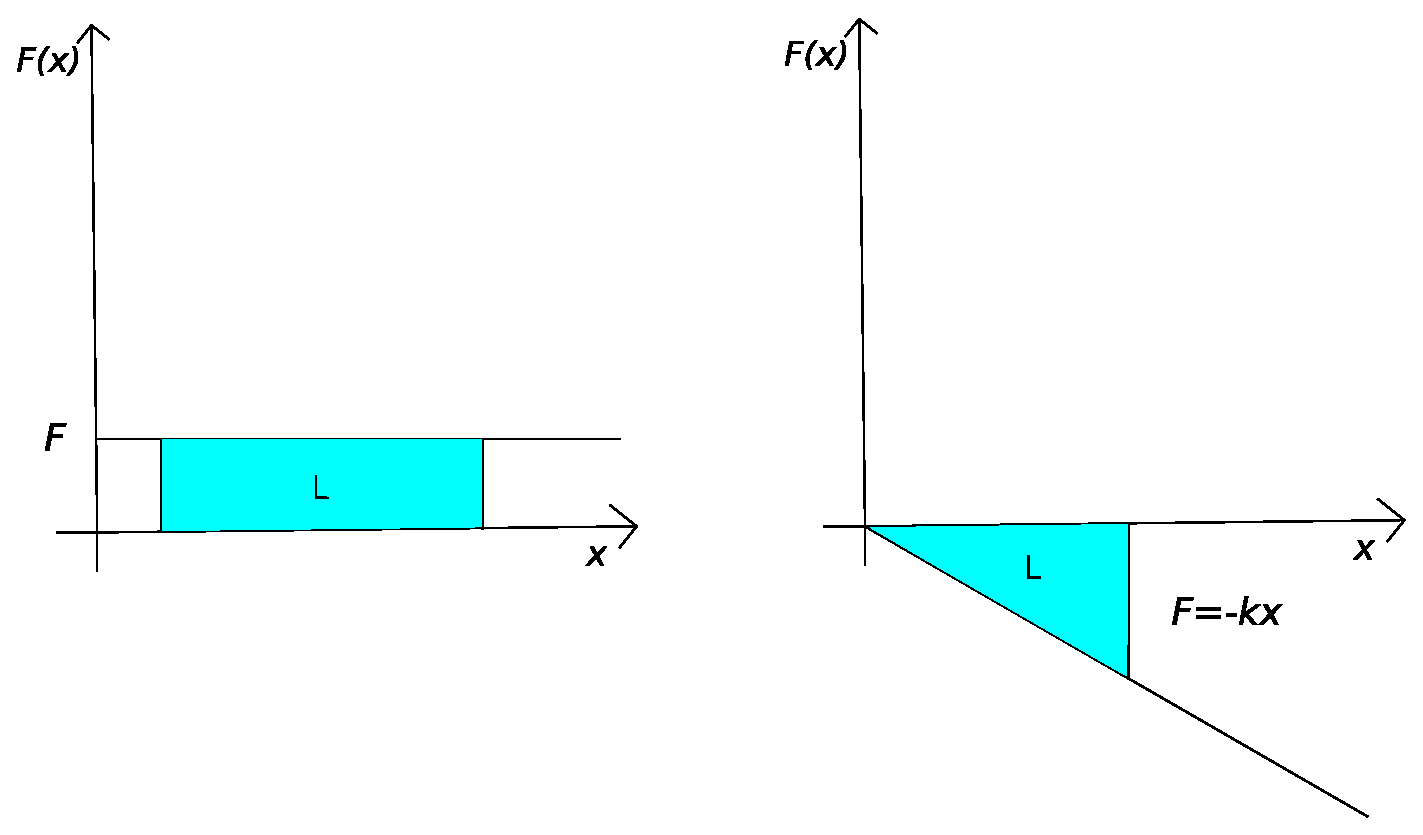
\includegraphics[width=8cm]{img/finiti/forze_costanti_e_elastiche.eps}
    \caption{Forze costanti e elastiche}
  \end{figure}
\end{defi}
\begin{nota}
  Nel caso della figura a sinistra si tratta di una forza costante, mentre, quella di destra è una
  forza elastica, come si vede nel caso della prima si presenta come un rettangolo che per
  l'appunto mantiene un intensità costante, mentre nel caso del secondo, ha un andamento che segue
  la funzione $F= -kx$
\end{nota}
\subsubsection{Lavoro della forza variabile prodotta dalle molle (Forza elastica)}
\begin{figure}[th]
    \centering
    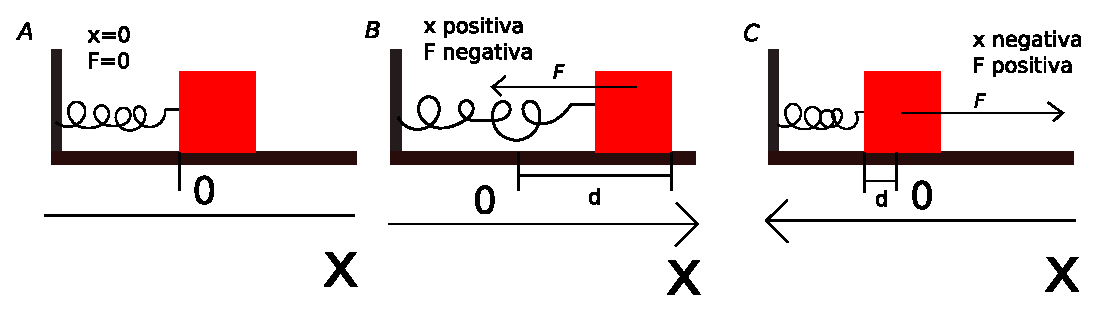
\includegraphics[width=10cm]{img/finiti/forza_elastica.eps}
    \caption{Forza elastica}
\end{figure}
\begin{equation}
  L_T=\int^{x}_0 \vec{F}_x*d\vec{x}=\int^x_0(-kx)dx=-1/2kx^2
\end{equation}

\begin{esempio}
  Calcolare il lavoro fatto dalla forza elastica di una molla avente $k=450\frac{N}{m}$ quando
  essa è stirata di 15 cm rispetto alla  sua posizione di riposo.
  \begin{equation}
    L_{F_e}= -1/2 kx^2=-0,5 * 450 \frac{N}{m}*(0,15m)^2=-5,06Nm=-5,06J
  \end{equation}
\end{esempio}
\clearpage
\subsection{Teorema dell’Energia Cinetica (caso unidimensionale forza costante)}
Consideriamo una forza $\vec{F}$ costante che agisce un corpo di massa m che sposta il suo punto di
applicazione di una quantità $\vec{s}$
\begin{figure}[th]
    \centering
    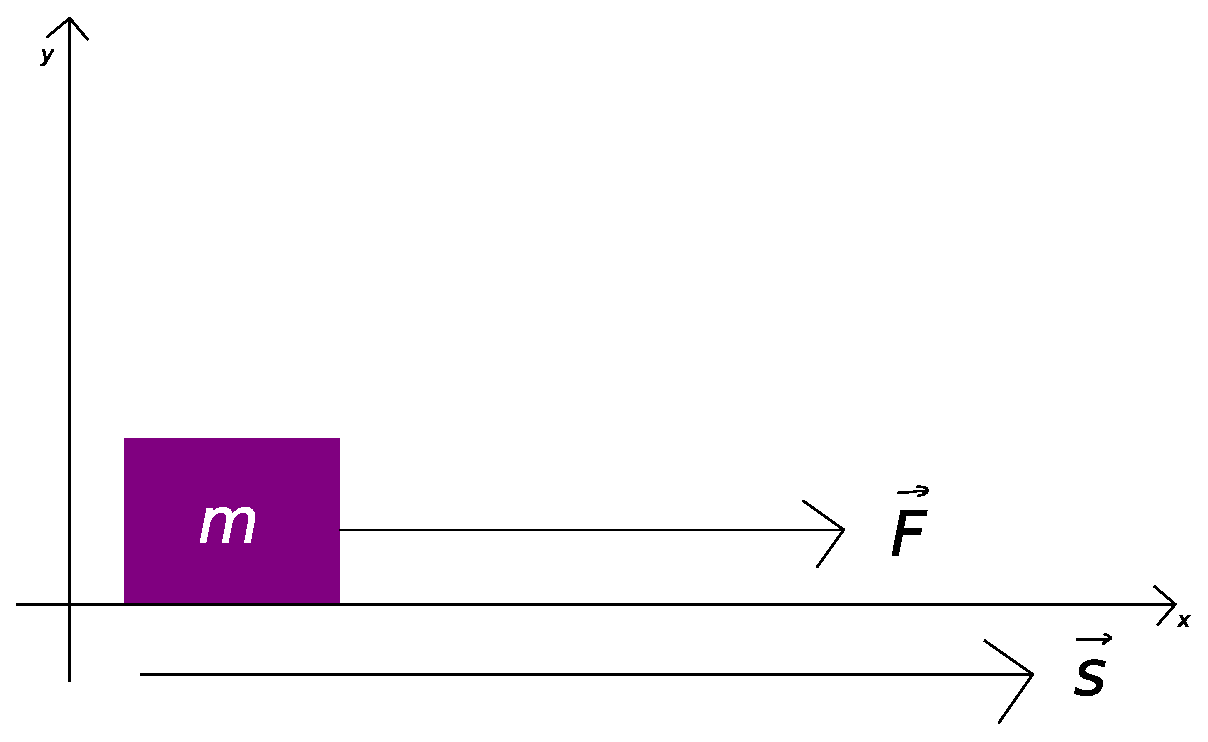
\includegraphics[width=10cm]{img/finiti/forza_costante.eps}
    \caption{Forza costante}
\end{figure}
\begin{equation}
  \begin{matrix}
    F=ma & a=\frac{F}{m}=costante \Rightarrow \text{ Moto naturalmente accelerato}
  \end{matrix}
\end{equation}
Abbiamo quindi che $v_2^2+2a(x_2-x_1)$ \footnote{Dove ($x_2-x_1$) è il modulo dello spostamento}
\begin{equation}
  L=\vec{F} * Fs \cos 0 = ma (x_2-x_1)=m\frac{v_2^2-v_1^2}{2(x_2-x_1)}(x_2-x_1)
\end{equation}
\begin{teo}
  In fisica, il teorema dell'energia cinetica (o teorema lavoro-energia, o
  teorema delle forze vive) afferma che se un corpo possiede un'energia cinetica iniziale e
  una forza agisce su di esso effettuando un lavoro, l'energia cinetica finale del corpo è
  uguale alla somma dell'energia cinetica iniziale e del lavoro compiuto dalla forza lungo
  la traiettoria del moto.
  \begin{equation}
    L=\frac{1}{2} m v_2^2-\frac{1}{2} m v_1^2=K_2-K_1=K_f-K_i=\Delta K
  \end{equation}
\end{teo}
\subsection{Lavoro di una forza variabile in 3 dimensioni}
\begin{figure}[th]
    \centering
    \includegraphics[width=6cm]{img/finiti/forza_vet_3d.eps}
    \caption{Forza vettoriale in 3 dimensioni}
\end{figure}
\begin{eqnarray*}
	\vec{S}=\displaystyle\sum_{i=1}^{N}\vec{S}_i & \begin{matrix}
		\text{Spostamento totale}\\
		\text{come limite della spezzata per}\\
		N\to \infty
	\end{matrix}\\
	& \vec{F}=F_x\vec{i}+\vec{F}_y\vec{j}+\vec{F}_z\vec{k}\\
	& d\vec{s}=dx\vec{i}+dy\vec{j}+dz\vec{k}
\end{eqnarray*}
Quindi si può dire che $L_T=\displaystyle\sum_{i=1}^{N}\vec{F}_i*\vec{s}_i\to
L_T=\int_{A}^{B}\vec{F}*d\vec{S}$, se e solo se $\abs{\vec{s}_i}\to 0$
\subsubsection{Teorema dell'energia cinematica tridimensionali}
\begin{eqnarray*}
	\vec{F}=F_x\vec{i}+\vec{F}_y\vec{j}+\vec{F}_z\vec{k}
	& d\vec{s}=dx\vec{i}+dy\vec{j}+dz\vec{k}
\end{eqnarray*}
\begin{eqnarray*}
	L=\int \vec{F}*d\vec{s}=\int
	\left(F_xd_x+F_yd_y+F_zdz\right)=\int_{x_1}^{x_2}ma_xdx+\int_{y_1}^{y_2}
	ma_ydy+\int_{x_1}^{z_2}ma_zdz\\ = \int_{x_1}^{x_2}m\frac{dv_x}{dt}dx+
	\int_{y_1}^{y_2}m\frac{dv_y}{dt}dy+\int_{z_1}^{z_2}m\frac{dy_z}{dt}dz=
	\int_{v_{x_1}}^{v_{x_2}}mv_xdv_x+\int_{v_{y_1}}^{v_{y_2}} mv_ydv_y
	+\int_{v_{x_1}}^{v_{z_2}}mv_zdv_z\\
	=\frac{1}{2}m\left[v_x^2\right]_{v_{x_1}}^{v_{x_2}}+ 
	\frac{1}{2}m\left[v_y^2\right]_{v_{y_1}}^{v_{y_2}}+\frac{1}{2}m
	\left[v_z^2\right]_{v_{z_1}}^{v_{z_2}}=
	\frac{1}{2}m\left[v_{x_2}^2-v_{x_1}^2\right]+
	\frac{1}{2}m\left[v_{y_2}^2-v_{y_1}^2\right]+
	\frac{1}{2}m\left[v_{z_2}^2-v_{z_1}^2\right]\\
	=\frac{1}{2}m\left[v_{x_2}^2+v_{y_2}^2+v_{z_2}^2\right]
	-\frac{1}{2}m\left[v_{x_1}^2+v_{y_1}^2+v_{z_1}^2\right]=\frac{1}{2}mv_2^2
	-\frac{1}{2}mv_1^2
\end{eqnarray*}
Quindi alla fine il risultato è 
\begin{equation*}
	\boxed{L=\frac{1}{2}mv_2^2
	-\frac{1}{2}mv_1^2}
\end{equation*}
Il lavoro fatto dalla forza ({\it risultante}) applicata al sistema è quindi
legato alla variazione della velocità del sistema durante l’applicazione della
forza stessa.
\section{Teorema dell'energia cinetica}
\begin{defi}
	L'energia cinetica è l'energia che possiede un corpo per il movimento che ha
	o che acquista: equivale al lavoro necessario per portare un corpo da una 
	velocità nulla a una velocità nota. Quando un corpo di massa m varia la sua 
	velocità, con questa varia anche la sua energia cinetica. Il lavoro equivale
	a questa variazione di energia cinetica. L'energia cinetica quindi è
	associata alla massa e alla velocità di un corpo in movimento. L'energia
	cinetica che possiede un corpo di massa m nel suo moto di caduta è uguale al
	lavoro compiuto per fermarsi.
\end{defi}
Matematicamente, l'energia cinetica è $K=\frac{1}{2}mv^2$ -- Il lavoro totale
fatto dalle forza che agiscono sul sistema considerato, è uguale alla
variazione della sua energia cinematica:
\begin{equation*}
	\boxed{L_T=L=\frac{1}{2}mv_2^2-\frac{1}{2}mv_1^2=K_2-K_1=K_f-K_i=\Delta K}
\end{equation*}
L'energia cinetica è uno scalare che ha le stesse dimensioni del Lavoro. Si
misura quindi in Joule ({\tt J})
\begin{equation*}
	[K]=[ML^2T^{-2}] \text{ Unità di misura: Joule (J)}
\end{equation*}
Lavoro ed Energia cinetica
\begin{eqnarray*}
	L_T>0\Rightarrow \Delta K>0 &v_f>v_i & \text{Il sistema accelera}\\
	L_T=0\Rightarrow \Delta K=0 &v_f=v_i & \text{La velocità del sistema rimane
	invariata}\\
	L_T<0\Rightarrow \Delta K<0 &v_f<v_i & \text{Il sistema decelera}
\end{eqnarray*}
\section{Lavoro ed energia}
\begin{esempio}
  Un blocco di massa $m=5kg$ viaggia con velocità costante pari a $7,6\frac{m}{s}$
  \begin{enumerate}
  \item Qual'è la sua energia cinetica?
  \item Quale lavoro totale è stato necessario fornirgli, se esso era inizialmente
    fermo, per portario a quella velocità?
  \item Quale lavoro totale è necessario per rallentarlo sino alla velocità di
    $4\frac{m}{s}$?
  \end{enumerate}
  \begin{enumerate}
  \item energia cinetica:
    \begin{equation*}
      K=\frac{1}{2}mv^2=0,5\times 5kg \times \left(7,5\frac{m}{s}\right)^2=140,6 Joule
      \cong 140,6J
    \end{equation*}
  \item Lavoro totale:
    \begin{equation*}
      L_T=\Delta K=\frac{1}{2}-\frac{1}{2}mv_1^2=[0,5\times 5kg\times (7,5\frac{m}{s})]=
      40J-141J=-101J
    \end{equation*}
  \end{enumerate}
\end{esempio}
\section{Forze conservative}
\begin{figure}[th]
    \centering
    \includegraphics[width=5cm]{img/finiti/forza_conservativa.eps}
    \caption{Forza conservative}
\end{figure}
Per una forza risulta che:
\begin{equation}
  L_{\gamma_1,A\to B}=\int_A^B \vec{F}*d\vec{s}=L_{\gamma_2,A\to B}
\end{equation}
è se il lavoro per andare da $A$ a $B$ non dipende dal corso seguito, allora diciamo che
la forza è \underline{Conservativa}.
\begin{figure}[th]
    \centering
    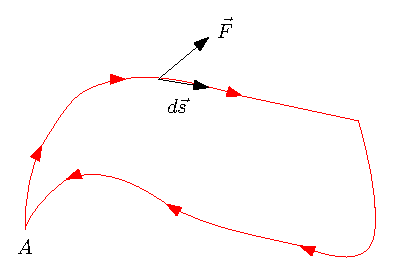
\includegraphics[width=5cm]{img/finiti/forza_conservativa_2.eps}
    \caption{Forza conservative}
\end{figure}
Se una forza è conservativa si ottiene anche che:
\begin{equation}
  L_{A\to A} =\oint \vec{F}*d\vec{s}=0
\end{equation}
\begin{esempio}
  Forza peso ({\tt forza gravitazionale})
 \begin{figure}[th]
    \centering
    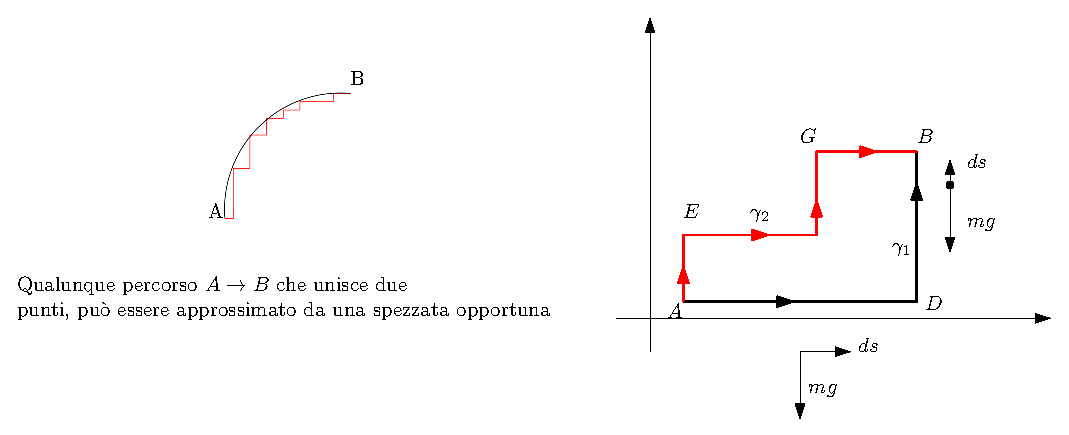
\includegraphics[width=15cm]{img/finiti/forza_peso.eps}
    \caption{Forza gravitazionale}
  \end{figure}
  \begin{equation}
    L_{\gamma_1,A\to B}=\int_{y_a}^{y_b}(-mg)dy+\int_{y_a}^{y_b}(-mg)dy=-mg(y_b-y_a)
  \end{equation}
  \paragraph{Analogamente:}
  \begin{align*}
    L_{\gamma_2,A\to B}=\int_{y_a}^{y_b}(-mg)dy=\int_{y_e}^{y_f}(-mg)dy+
    \int_{y_f}^{y_g}(-mg)dy+\int_{y_g}^{y_b}(-mg)dy=-mg(y_b-y_a)\\=
    \int_{y_a}^{y_b}(-mg)dy=-mg(y_b-y_a)
  \end{align*}
  \paragraph{Conclusioni:} $L_{\gamma_1,A\to B}=L_{\gamma_2,A\to B}$ La Forza peso
  (forza gravitazionale) è conservativa!
\end{esempio}
\begin{esempio}
  Forza Elastica
  \begin{figure}[th]
    \centering
    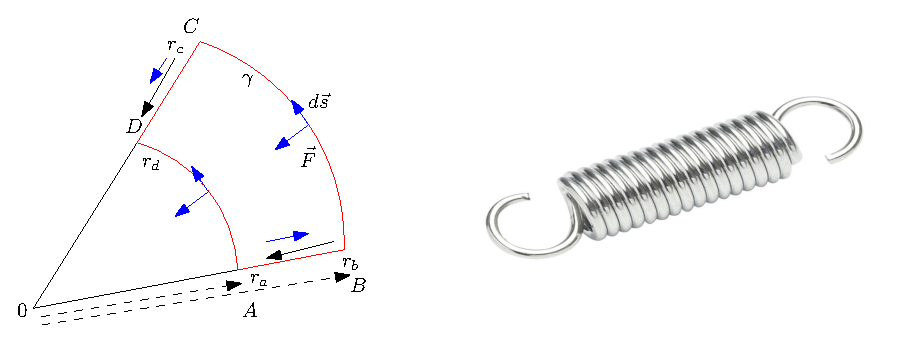
\includegraphics[width=10cm]{img/finiti/forza_elastica_es.eps}
    \caption{Forza elastica}
  \end{figure}
  \begin{eqnarray*}
    L_{A\to B}=\int_{A}^{B}\vec{F}_e*d\vec{s}=\int_{r_a}^{r_b} -krdr=-\frac{1}{2}k
    [r_b^2-r_a^2]\\
    L_{B\to C}=\int_{B}^{C}\vec{F}_e*d\vec{s}=0\\
    L_{C\to D}=\int_{C}^{D}\vec{F}_e*d\vec{s}=\int_{r_c}^{r_d} -krdr=-\frac{1}{2}k
    [r_d^2-r_c^2]=+\frac{1}{2}k [r_c^2-r_d^2]\\
    L_{D\to A}=\int_{D}^{A}\vec{F}_e*d\vec{s}=0
  \end{eqnarray*}
  Essendo $r_c=r_b$ e $r_a=r_d$ si ha che:
  \begin{equation}
    L_{A\to A}\oint_\gamma \vec{F}* d\vec{s}=L_{A\to B}+L_{B\to C}+L_{C\to D}+L_{D\to A}
  \end{equation}
  {\tt Per questo motivo la forza elastica è conservativa}
\end{esempio}